\documentclass[10pt]{sigplanconf}
\usepackage{amsfonts}
\usepackage{amsmath}
\usepackage{amssymb}
\usepackage{graphicx}
\usepackage{fancyvrb}
\usepackage{listings}
\usepackage{eqntabular}
\usepackage{renumber}
\usepackage{galois}

\newtheorem{definition}{Definition}
\newtheorem{example}{Example}


\newcommand\codefamily\ttfamily
\lstset{language={[Sharp]C},mathescape=false,flexiblecolumns=true,morekeywords={Contract},basicstyle=\codefamily\small,moredelim=[is][\itshape]{@}{@},captionpos=b,numberstyle=\tiny,stepnumber=1,numbersep=2pt,keywordstyle=\bfseries}

\lstset{boxpos=t}

%% Macros
\newcommand{\labelSection}[1]{\label{sec:#1}}
\newcommand{\labelFig}[1]{\label{fig:#1}}
\newcommand{\labelDef}[1]{\label{def:#1}}

\newcommand{\refSection}[1]{Sec.~\ref{sec:#1}}
\newcommand{\refFig}[1]{Fig.~\ref{fig:#1}}
\newcommand{\refDef}[1]{Definition ~\ref{def:#1}}

\newcommand{\code}[1]{\texttt{#1}}

\newcommand{\clousot}{\code{cccheck}}
\newcommand{\Clousot}{\code{Cccheck}}

%% Math Macros
\newcommand{\ltuple}[1]{\langle#1,\allowbreak}
\newcommand{\mtuple}[1]{\:#1,\allowbreak}
\newcommand{\rtuple}[1]{\:#1\rangle}
\newcommand{\pair}[2]{\ltuple{#1}\rtuple{#2}}

\newcommand{\diff}[2]{\delta_{\code{#1}, \code{#2}}}

\newcommand{\emptytrace}{\vec{\epsilon}}
\newcommand{\seqcomp}{\dot}
\newcommand{\length}[1]{\mathopen{{|}}\mskip1mu#1\mskip1mu\mathclose{{|}}}
\makeatletter
\newcommand{\pvec}[1]{\overline{\vec{#1}}}
\makeatother

% page numbering
\pagestyle{plain}

\title{Modular and Verified Automatic Program Repair}

\authorinfo{Francesco Logozzo \and Thomas Ball}
{Microsoft Research, Redmond}
{\{ logozzo, tball\} @microsoft.com}

\begin{document}
\conferenceinfo{OOPSLA'12,} {October 19--26, 2012, Tucson, Arizona, USA.}
\CopyrightYear{2012}
\copyrightdata{978-1-4503-1561-6/12/10}
\maketitle

\begin{abstract}

We study the problem of suggesting code repairs at \emph{design time},
based on the warnings issued by modular program verifiers. We
introduce the concept of a \emph{verified} repair, a change to a program's
source that removes bad execution traces while increasing the number
of good traces, where the bad/good traces form a partition of all the
traces of a program. Repairs are property-specific. We demonstrate our
framework in the context of warnings produced by the modular \clousot~(a.k.a. \code{Clousot})
abstract interpreter, and generate repairs for missing contracts,
incorrect locals and objects initialization, wrong conditionals,
buffer overruns, arithmetic overflow and incorrect floating point
comparisons.  We report our experience with automatically generating
repairs for the .NET framework libraries, generating verified repairs
for over 80\% of the warnings generated by \clousot.

\end{abstract}

\category{D. Software}{D.1 Programming Techniques}{D.1.0 General,  D.2.1 Requirements/Specifications, D.2.2 Design Tools and Technique, D.2.4 Software/Program Verification D.2.5 Testing and Debugging D.2.6 Programming Environments}

\terms{Design,
    Documentation,
    Experimentation,
    Human Factors,
    Languages,
    Reliability,
    Verification. }

\keywords{Abstract interpretation, Design by contract, Program repair, Program transformation, Refactoring, Static analysis.}\


\section{Introduction}

Programs have bugs. Sound static analyzers, such as automatic program
verifiers, can catch bugs but usually leave the problem of repairing
the program to the developer.  During active development, reports of
possible bugs may be of little interest to programmers. On the other
hand, if a program verifier can suggest code repairs, it can
potentially help the programmer write correct code.

We focus on the problem of suggesting code repairs starting from the
warning issued by a  modular program verifier. 
A modular verifier uses contracts (\emph{i.e.}, preconditions, postconditions,
and object invariants) to
decompose the verification problem from the level of a whole program
to the level of individual methods.  Developer-supplied contracts are
essential not only for scalability but also for documenting intent as
well as localizing the cause of failures~\cite{MeyerIEEEComputer92}.

The first step in addressing the problem is to focus attention on the
bugs that matter to developers. 
In our case, we consider contract violations and runtime errors.
A tool like \clousot~\cite{cccheck}, the CodeContracts static checker, can spot those errors at design time.
Ideally, \clousot\ should not only report the warnings, 
but also provide a (set of) possible fixes, that are
then presented to the programmer to choose among or reject.

The second step in addressing the problem is to define what a code
repair is. Previous work on automatic program repair by Perkins
\emph{et al.}~\cite{PerkinsEtAl09} defines a repair to be a code
transformation such that the repaired program passes a given set of
test cases (including the one exposing the bug). This definition is
not well-suited to the context of verification and active program
development as it requires running the repaired program, which may not
always be possible, and it is only as good as the given regression
test suite.

Because of these limitations and our desire to statically reason about
program defects and repairs, we propose a different definition for
repair. A \emph{verified} repair reduces the number of
\emph{bad} executions in the program, while preserving, or 
increasing, the number of \emph{good} runs.  A bad run is one that
violates a given specification (assertion, precondition, run-time
guard, etc.).  A good run is one that meets all specifications of
the original program. These two sets of traces form a partition of
{\em all the traces} of a program.


\begin{figure*}[th]
\centering
\begin{tabular}{l|l}
\begin{lstlisting}
void P(int[] a)
{


  for (var i = 0; i < a.Length; i++)
    a[i - 1] = 110;
}
\end{lstlisting} &
\begin{lstlisting}
void P'(int[] a)
{
  Contract.Requires(a != null);

  for (var i = 1; i < a.Length; i++)
    a[i - 1] = 110;
 }
\end{lstlisting}
\end{tabular}
\caption{\Clousot\ detects the possible null-dereference of \code{a} and a definite buffer underflow in  \code{P}.  
It suggests the precondition \code{a != null} and initializing
\code{i} to $1$.  The resulting correct program is \code{P'}.}
\labelFig{ForExample}
\end{figure*}


Using abstract interpretation, we design a general framework in which code repairs can be expressed.
We define several abstractions of trace semantics in order to permit a wide variety of program repairs. 
One abstraction restricts what is observable about program state to the
program points containing assertions, which is necessary since we
expect program repairs to change the control flow of programs. 
A Boolean abstraction further restricts the observations to the Boolean values of assert expressions, which permits changes to program variables appearing in the program and the assertion expression itself.
Based on this semantic foundation, one can design different algorithms for code repairs.
In general there is no unique recipe for designing verified code repairs, in the same way as in abstract interpretation there is no unique way of designing abstract domains.

We relate the problem of designing code repairs to program verification/analysis as follows.
There are three components in program analysis: the program, the semantic knowledge about program behavior, and the property to be verified.
In program analysis, the problem is to refine the semantic knowledge so to derive that the properties hold for the program (verification) or do not hold (bug finding).
In code repairs, the problem is to \emph{refine the program} using the semantic knowledge so that it satisfies the properties of interest.
In \clousot, or similar tools, the semantic knowledge is given by the abstract state, belonging to some abstract domain, which was computed by the analysis.
The next natural step is to exploit the abstract state to derive the semantic code fix.
Therefore, code repairs are \emph{domain-dependent}.
We envision code repairs to be standard part of the design of static analyses, abstract domains and verification systems in general.

\paragraph{Main contributions}
We define the notions of verified repairs in terms of abstractions of trace semantics.
We present \emph{sound} algorithms
for suggesting program repairs to: contracts
(preconditions, postconditions, assumptions, pure methods),
initialization (wrong constants, buffer size, object fields), guards
(negation, strengthening, weakening),  buffer overflows, floating
point comparisons, and overflowing expressions.  While we use
\clousot\ as our verifier, the proposed
repairs can be easily adapted and implemented in most any  static analyzer.

It is worth noting that our formalization of verified repairs is with
respect to the specifications of the original program. As we will see,
some repairs are verified by construction. For others, we need to
apply the repair and check the repaired program to ensure it does not
violate other assertions, \emph{i.e.}, we want to avoid the situation where repairing an assertion causes the failure of another assertion downstream.
The fact that all repairs are local to a method means that verifying a repair only requires
local analysis and can be applied to incomplete programs.
In general, for a given warning, several distinct repairs are possible.
Repairs can be ranked according to some metric of interest, \emph{e.g.}, complexity, size of the change, \emph{etc.}
We show that the local analysis is very fast -- in the order of $150ms$ per method -- and  that the repair inference is just a tiny portion of that time.
We can infer thousands of repairs in large C$\#$ libraries and we can propose a repair for more than $80\%$ of the warnings issued by the analyzer. 
We are confindent that our code repairs can be used in an interactive IDE.

\paragraph{Plan} The remainder of the paper is organized as
follows. Section~\ref{sec:examples} illustrates the kind of repairs we
are able to produce automatically.  Section~\ref{sec:tracesemantics}
presents a trace-based semantics of programs. 
Section~\ref{sec:verifiedrepairs} defines abstractions over traces and  formalizes two kinds of verified repairs.
Section~\ref{sec:fromStaticAnalyzer} extends those abstractions when a static analyzer is used.
Section~\ref{sec:fixespractice} describes the
\clousot\ verifier, the types of errors it can find, and the specific
repairs enabled by \clousot.  
Section~\ref{sec:experience} discusses our experience with automatically repairing very large C\# programs,
Section~\ref{sec:related} reviews related work and
Section~\ref{sec:conclude} concludes the paper.

\section{Examples of Program Repairs}
\label{sec:examples}

\paragraph{Repair by Contract Introduction.} 
It is often the case that the code of a method is correct only when
executed under certain conditions.  In the example
of~\refFig{ForExample}, when the parameter \code{a} is null, there
will definitely be a failure due to a null dereference of the
parameter.  In this case, the \Clousot\ tool suggests the precondition
\code{a != null} using a \code{Requires} contract~\cite{CousotCousotLogozzo-VMCAI11}.

In the example of~\refFig{AssumeExample}, when \code{length} is
negative, the array allocation will always fail.  In this case, there
are two possible repairs: (i) add an explicit assumption \code{0 <=
length}; or (ii) add the postcondition to \code{GetALength} stating it
will always return a non-negative value.  \Clousot\ suggests both to
the programmer and lets her choose which one to apply.  The first
repair is useful when \code{GetALength} is a third-party or external
code, as it makes the programmer assumption explicit and prevents
\Clousot\ from generating a warning. The second repair documents 
the behavior of \code{GetALength}, clearly stating the contract
clients of the method can rely upon.

In this example, both a buffer underflow and overflow are possible.
In these cases, \Clousot\ proposes the precondition~\code{0 <= index}
and the assumption
\(
\code{Assume}\allowbreak \code{(index}\allowbreak \code{ < length)}
\),
making explicit
the relationship between the return value of~\code{GetALength} and the
parameter \code{index}.

%\Clousot\ also infers and suggests adding object invariants to state invariants on object fields~\cite{Logozzo-VMCAI07}.

\begin{figure}
\begin{lstlisting}
int[] ContractRepairs(int index)
{
  var length = GetALength(); // (1)
  var arr = new int[length]; 
  arr[index] = 9876;
  return arr;
 }
\end{lstlisting}

\caption{\Clousot\ spots several possible errors in the code (allocation of an array of negative size, buffer overruns).  
See the paper text for a description the proposed repairs.}
\labelFig{AssumeExample}
\end{figure}




\paragraph{Repair of Initialization and Off-By-One Errors.} 
Another class of errors arises from the improper initialization of
variables (especially loop induction variables) or use of constants
just outside a safe zone.  In the for loop of~\refFig{ForExample},
\Clousot\ detects a buffer underflow and localizes the cause to be in
the initialization of \code{i}.  
\Clousot\ infers that: (i) the constraint $0 < \code{i}$ should hold on  loop entry; and (ii)  any positive initial value for \code{i} removes the buffer undeflow.
The initialization $\code{i} = 1$ is the one that enables most good runs, and it is therefore the one suggested to the user.
In the example of~\refFig{ArrayInitExample},
\Clousot\ detects a buffer underflow and suggests two potential
repairs: allocate a buffer of length at least $2$; use $0$ to index
the array (to avoid the buffer overflow, without introducing an
underflow).

\begin{figure}
\begin{lstlisting}
string GetString(string key)    
{
 var str = GetString(key, null);
 if (str == null)
 {
  var args = new object[1];
  args[1] = key; // (*)
  throw new ApplicationException(args);
 }
 return str;
}
\end{lstlisting}
\caption{A (simplified) code snippet from  \code{CustomMarshalers.dll}.
\Clousot\ detects the buffer overrun at \code{(*)}, and suggests the allocation of a larger buffer at the line above or changing the index to $0$.}
\labelFig{ArrayInitExample}
\end{figure}

\begin{figure}[t]
\begin{lstlisting}
void ValidateOwnerDrawRegions(
  ComboBox c, Rectangle updateRegionBox)
{
  if (c == null)
  {
    var r = new Rectangle(0, 0, c.Width); // (*)
   // use r and c
  }
}
\end{lstlisting}
\caption{A (simplified) snippet from a bug found in \code{System.Windows.Forms.dll}. 
\clousot\ proposes the repair \code{c != null} as a precondition or as a replacement
for the guard of the if-then statement.}
\labelFig{NNExample}
\end{figure}

\begin{figure}[t]
\begin{lstlisting}
IMethodCallMessage ReadArray(
   object[] callA, object handlerObject)
{
  if (callA == null) return null;
  var num = 0;
  if (NonDet())) num++; 
  if (callA.Length < num) 
    throw new SerializationException();

  // here callA.Length >= num
 
  this.args = (object[])callA[num++];
   // ...
}
\end{lstlisting}
\caption{A (simplified) snippet from a bug found \code{mscorlib.dll}. 
\Clousot\ proposes to change the guard to \code{callA.Length <= num}}
\labelFig{Strengthening}
\end{figure}

\paragraph{Repairing Guards of Conditional Statements.} 
Let us consider the code snippet in ~\refFig{NNExample}, taken from one of the .NET framework libraries.
At program point \code{(*)}: (i) \code{c != null} should hold, otherwise the program will crash with a null-pointer exception;
(ii) \clousot\ determines that  \code{c} is \code{null} for all the executions reaching that point (a definite error).
\Clousot\ suggests three repairs: the \emph{necessary} precondition \code{c != null};
flipping the guard from \code{c == null} to \code{c != null}; removing the branch altogether.
 Note that neither repair removes any \emph{good} trace present in the original program, but does remove bad traces.
Also, there is no \emph{best} repair. 
We do not rank repairs: we simply report them at the program point where they should be applied.

In~\refFig{Strengthening}, \clousot\ suggests to strengthen the
\code{if}-guard to the condition \code{callA.Length <= num}, as a buffer 
overflow may happen otherwise (a \code{Serialization} exception is not
considered an error).



\begin{figure}[t]
\begin{lstlisting}
class FloatingPoint
{
 double d;

 [ContractInvariantMethod]
 void ObjectInvariant()
 {
  Contract.Invariant(this.d != 0.0);
 }

 public void Set(double d0)
 {
  // here d0 may have extended double precision 
  if (d0 != 0.0) 
    this.d = d0; // d0 can be truncated to 0.0
  }
}
\end{lstlisting}
\caption{A (simplified) snippet from a bug found \code{mscorlib.dll}. 
The store field causes the truncation of \code{d0} which may break the invariant, despite the guard.
\Clousot\ proposes repairing the guard by adding the truncation to \code{d0}.}
\labelFig{FloatingPointExample}
\end{figure}

\paragraph{Repairing Erroneous Floating Point Comparisons.}
Floating point comparisons may produce unexpected
results~\cite{LogozzoFahndrich11}.  The .NET semantics enforces the
runtime to use: (i) for stack values, the most precise floating point
representation available from the hardware; (ii) for heap values, the
representation exactly matching the nominal type.  In the code
of~\refFig{FloatingPointExample}, the parameter \code{d0} may be a
very small, non-zero double represented by $80$ bits on \code{x86}.
The test succeeds, but the next assignment causes the truncation of
the value of \code{d0} to a $64$-bit quantity, that may be zero,
violating the object invariant. \Clousot\ identifies the problem and
suggests repairing the guard to \code{(double)d0 != 0.0}, \emph{i.e.},
forcing the comparison of the $64$-bit truncation of \code{d0} to
zero.  


\begin{figure}[t]
\begin{lstlisting}
int BinarySearch(int[] array, int value)
{
  Contract.Requires(array != null);
  int inf = 0, sup = array.Length - 1; 

  while (inf <= sup)
  {
   var index = (inf + sup) /2 ; // (*)
   var mid = array[index];

   if (value == mid) return index;
   if (mid < value)  inf = index + 1; 
   else              sup = index - 1;
  }
  return -1;
}
\end{lstlisting}
\caption{\Clousot\ detects and automatically proposes a repair for overflow 
in the computation of the variable \code{mid}, using the loop
invariants automatically inferred by the abstract interpreter.}
\labelFig{OverflowExample}
\end{figure}

\begin{figure}[t]
\begin{lstlisting}
void ThreadSafeCopy(char* sourcePtr, char[] dest, 
                    int destIndex, int count)
{
 if (count > 0)
   if ((destIndex > dest.Length) 
    || ((count + destIndex) > dest.Length))
      throw new ArgumentOutOfRangeException();
   { // ... } 
}
\end{lstlisting}
\caption{A code snippet from a bug in \code{mscorlib.dll}. 
\Clousot detects that \code{count + destIndex} may overflow and suggests repairing
the expression to the non-overflowing \code{count > dest.Length - destIndex}.}
\labelFig{OverflowExample2}
\end{figure}

\paragraph{Repairing Overflowing Expressions.}
Verified repairs are very helpful for dealing with unintended
arithmetic overflows.  Consider the classical binary search example
of~\refFig{OverflowExample}: The expression at \code{(*)} may
overflow, setting \code{index} to a negative value, causing a buffer
underflow in the next line.
\Clousot\ suggests repairing the expression to \code{inf + (sup - inf) / 2},
which: (i) allows more good runs (inputs that previously caused
the overflow now are ok); (ii) is based on the loop invariant
automatically discovered by \clousot: $0 \leq
\code{inf} \leq \code {sup} < \code{array.Length}$.  

In the example of~\refFig{OverflowExample2}, \code{count} can be a
very large positive value, causing \code{count + destIndex} to
overflow. \Clousot\ suggests repairing the expression to \code{count >
dest.Length - destIndex}.

\section{Trace Semantics}
\label{sec:tracesemantics}

We formalize the notion of a verified program repair via a trace
semantics.  As we are only interested in repairs of violations of
safety properties, we only consider finite traces.

Let \code{P} be a program.
\code{P(pc)} denotes the statement at program point \code{pc}, and $\code{P}[\code{pc} \mapsto \code{S}]$ denotes 
the program that is the same as \code{P} everywhere except \code{pc}, where it contains the statement \code{S}.
If \code{S} is a compound statement, a remapping of \code{S}'s program points may be needed.
We keep the remapping implicit to simplify the notation.
We let $\mathbb{E}$ denote the set of  pure Boolean expressions.  

Let $\Sigma$ be a set of states, and $\tau_\code{P} \in \wp(\Sigma \times \Sigma)$ be a non-deterministic transition relation.
For a state $s \in \Sigma$, $s(\code{C})$ denotes the basic command associated with the state, \emph{e.g.}, an assignment, an assumption, or an assertion.
The set of blocking states, \emph{i.e.}, states with no successors, is  $\mathfrak{B} = \{ s \in \Sigma \mid \forall s'.\ \neg \tau_\code{P}(s, s')\}$.
The set of erroneous state, \emph{i.e.}, states violating some assertion $\code{e}$, is $\mathfrak{E} = \{ s \in \Sigma \mid s(\code{C}) = \code{assert e} \wedge s \not\models \code{e}\} \subseteq \mathfrak{B}$.

Traces are sequences of states. 
Concatenation is denoted by juxtaposition and extended to sets of traces. 
$\vec{\Sigma}^n$ is the set of non-empty \emph{finite traces} $\vec{s}=\vec{s}_0\ldots\vec{s}_{n-1}$ of length $\length{\vec{s}} = n \geq 0$ including the \emph{empty trace} $\emptytrace $ of length $\length{\emptytrace} \triangleq 0$. 
$\vec{\Sigma}^+\triangleq\bigcup_{n\geqslant1}\vec{\Sigma}^n$  is the set of \emph{non-empty finite traces} and $\vec{\Sigma}^\ast =\vec{\Sigma}^+\cup\{\emptytrace\}$.  
The set of \emph{finite bad traces}, \emph{i.e.}, traces containing  an error is $\vec{\mathfrak{E}} = \{ \vec{s} \in \vec{\Sigma}^+ \mid \exists i \in [0, \length{\vec{s}}).\ s_i \in \mathfrak{E} \}$.
The bad (resp. good) traces of $T \subseteq \vec{\Sigma}^\ast$ are $\mathcal{B}(T) \triangleq T \cap \vec{\mathfrak{E}}$ (resp. $\mathcal{C}(T) \triangleq T \cap (\vec{\Sigma}^\ast \setminus \vec{\mathfrak{E}})$).
The function $\mu \in  \wp(\Sigma^\ast) \rightarrow \wp(\Sigma^\ast)$ filters the maximal traces out of a set of traces.
Given a set of traces $T$, $\mu(T)$ is the largest set satisfying the properties: $\mu(T) \subseteq T$ and $\forall \tau \in \mu(T). \not \exists \tau' \in T. \exists \tau''. \tau'' \neq \emptytrace \wedge \tau' = \tau \tau''$. 

The \emph{maximal  execution traces} or \emph{runs} are prefix traces generated by applying the transition relation from the initial states until a fixpoint is reached (partial execution traces) followed by a projection on the maximal traces:
\begin{eqntabular}{ll}\label{eq:fixpoint}
\vec{\tau}_\code{P}^+(S)  = \mu(\mathsf{lfp} \lambda T.\ S \cup \{  \sigma_0 \dots \sigma_n \sigma_{n+1}  \mid \\ 
\qquad \qquad \qquad \qquad \sigma_0 \dots \sigma_n \in T\wedge \tau(\sigma_n, \sigma_{n+1}) \}). \nonumber 
\end{eqntabular}

The \emph{bad (resp. good) finite complete runs}, or simply \emph{bad (resp. good) runs} of \code{P} are $\mathcal{B}_\code{P} \triangleq \mathcal{B}(\vec{\tau}^+_\code{P})$ (resp. $\mathcal{G}_\code{P} \triangleq \mathcal{G}( \vec{\tau}^+_\code{P})$).

The definitions above (and in the following) can be extended as in~\cite{Cousot-TCS02} to take into account infinite runs, but we avoid doing it here to keep the presentation as simple as possible. 


\section{Verified Repairs}
\label{sec:verifiedrepairs}
Hereafter, we assume that \code{P} is the program containing a bug and
\code{P'} the repaired version.  Intuitively, \code{P'} should have
more good runs and fewer bad runs than \code{P}.  Because a repair may
change the program's control flow, introducing new states, and
possibly new assertions, the concrete traces of
\code{P} and \code{P'} may appear very different. Thus,
the simple inclusions $\mathcal{G}_\code{P'} \supseteq
\mathcal{G}_\code{P}$ and $\mathcal{B}_\code{P'} \subseteq
\mathcal{B}_\code{P}$ may be too strict and hold only for trivial
repairs.

Instead, we compare the semantics of \code{P} and
\code{P'} at a higher level of abstraction.  First, we remove
all states but those containing assertion statements (the {\em
assertion trace semantics}).  Then, we remove all new assertions
introduced in \code{P'}.
Abstract interpretation~\cite{CousotCousot77} provides the right framework to formalize this.


\paragraph{Basic Elements of Abstract Interpretation.} 
We first recall some basic facts and notations about abstract interpretation.
A \emph{Galois connection} $\pair{L}{\leqslant}\galois{{\alpha}}{{\gamma}}\pair{\overline{L}}{\sqsubseteq}$ consists of posets $\pair{L}{\leqslant}$, $\pair{\overline{L}}{\sqsubseteq}$ and maps $\alpha\in L\rightarrow\overline{L}$, $\gamma\in\overline{L}\rightarrow L$ such that $\forall x\in L,y\in\overline{L}: \alpha(x) \sqsubseteq y\iff x\leqslant\gamma(y)$. 
In a Galois connection, the \emph{abstraction} $\alpha$ preserves existing least upper bounds (lubs) hence is monotonically increasing so, by duality, the \emph{concretization}  $\gamma$ preserves existing greatest lower bounds (glbs) and is monotonically increasing. 
The composition of Galois connections is a Galois connection.

\paragraph{Assertion Trace Semantics.}
The assertion abstraction $\alpha_\code{A}$ removes all states but those referring to assertions.
The abstraction $\alpha^1_\code{A} \in \vec{\Sigma}^\ast \rightarrow \vec{\Sigma}^\ast$ on a single trace:
\[
\alpha^1_\code{A}(\vec{s}) = \left\{
\begin{array}{l l}
  \emptytrace                 & \vec{s} = \emptytrace \\
  s\alpha^1_\code{A}(\vec{s'}) &  \vec{s} = s\vec{s'} \wedge s(\code{C}) = \code{assert e} \\
  \alpha^1_\code{A}(\vec{s'})  & \vec{s} = s\vec{s'} \wedge s(\code{C}) \not= \code{assert e}
\end{array}
\right.
\]
can be lifted to a set of traces $\alpha_\code{A} \in \wp(\vec{\Sigma}^\ast) \rightarrow \wp(\vec{\Sigma}^\ast)$: 
\(
\alpha_\code{A}(T) = \bigcup_{\vec{s} \in T} \alpha^1_\code{A}(\vec{s}).
\)
The function $\alpha_\code{A}$, is a complete $\cup$-morphism.
Thus, it exists a unique concretization $\gamma_\code{A}$ such that $\pair{\wp(\vec{\Sigma}^\ast)}{\subseteq}\galois{{\alpha_\code{A}}}{{\gamma_\code{A}}}\pair{\wp(\vec{\Sigma}^\ast)}{\subseteq}$~\cite{CousotCousot77}.
The \emph{assertion trace semantics} of \code{P} is $\alpha_\code{A}(\vec{\tau}^+_\code{P})$.

In general, a repair may introduce new assertions (that may or may not
hold).  As the goal of a repair is to address failing assertions of
the original program, we remove from the assertion semantics of
\code{P'} all the \emph{new} assertions and the \emph{new} variables
before comparing the behaviors of \code{P} and \code{P'}.

%If in \code{P'} an assertion was removed, it will \emph{not} appear in  $\mathbb{A}(\diff{P}{P'})$.

Let $\diff{P}{P'}$ denote a {\em repair} that transforms program
\code{P} to program \code{P'} and let $\mathbb{A}(\diff{P}{P'})$ be 
all the \emph{new} assertions introduced by the
repair in \code{P'}. Let $\pi_{\diff{P}{P'}} \in \Sigma \rightarrow
\Sigma$ denote the state projection over all the common variables of \code{P} and \code{P'}.
The function $\alpha^1_{\diff{P}{P'}} \in \vec{\Sigma}^\ast
\rightarrow \vec{\Sigma}^\ast$ removes all the new assertions and
new variables from a trace:
\[
\alpha^1_{\diff{P}{P'}}(\vec{s}) = \left\{
\begin{array}{l l}
  \emptytrace                 & \vec{s} = \emptytrace \\
  \pi_{\diff{P}{P'}}(s)\alpha^1_{\diff{P}{P'}}(\vec{s'}) & \vec{s} = s\vec{s'} \wedge s(\code{C}) \not \in \mathbb{A}(\diff{P}{P'}) \\
  \alpha^1_{\diff{P}{P'}}(\vec{s'})  &  \vec{s} = s\vec{s'} \wedge s(\code{C}) \in \mathbb{A}(\diff{P}{P'}) \\
\end{array}
\right.
\]
and its lifting to sets  $\alpha_{\diff{P}{P'}} \in  \wp(\vec{\Sigma}^\ast) \rightarrow \wp(\vec{\Sigma}^\ast)$, defined as 
\(
\alpha_{\diff{P}{P'}}(T) = \bigcup_{\vec{s} \in T} \alpha^1_{\diff{P}{P'}}(\vec{s}),
\)
is a complete $\cup$-morphism, so that it exists a concretization function $\gamma_{\diff{P}{P'}}$ such that $\pair{\wp(\vec{\Sigma}^\ast)}{\subseteq}\galois{{\alpha_{\diff{P}{P'}}}}{{\gamma_{\diff{P}{P'}}}}\pair{\wp(\vec{\Sigma}^\ast)}{\subseteq}$.

\paragraph{Verified Repairs.}
We are now ready to formally define the concepts of a {\em verified
repair} and a repaired program {\em improving} another program.

\begin{definition}[Verified repair, improvement]
\labelDef{SemanticFixes}
If $\alpha_\code{A}(\mathcal{G}_\code{P}) \subseteq \alpha_{\diff{P}{P'}} \circ \alpha_\code{A}(\mathcal{G}_\code{P'})$ and 
$\alpha_\code{A}(\mathcal{B}_\code{P}) \supset \alpha_{\diff{P}{P'}} \circ \alpha_\code{A}(\mathcal{B}_\code{P'})$, then we say that  $\diff{P}{P'}$ is a verified repair for \code{P} and that \code{P'} is an improvement of \code{P}.
\end{definition}

The above definition denies the identity (\emph{i.e.}, program \code{P}
itself) as a trivial improvement, since the number of bad traces should
strictly decrease.  It allows the removal of an \emph{always} failing
assertion as a repair.  If an assertion fails in some executions and
passes in others, then its removal is disallowed (as the subset
inclusion on good runs will fail).  For a given program
\code{P}, there may be several distinct improvements $\code{P'}_1,
\code{P'}_2 \dots$ (\emph{e.g.},~\refFig{AssumeExample}
or~\refFig{NNExample}).  
One can define an additional scoring function to rank $\code{P'}_1, \code{P'}_2 \dots$.
The definition of verified repair naturally
induces a partial order on programs (and hence on improvements): a
program \code{Q} improves \code{R}, written $\code{R} \sqsubseteq
\code{Q}$ if $\diff{R}{Q}$ is a verified repair for \code{R}.  We
only compare the ``same'' assertions over two versions of the program,
so \code{P'} may introduce new bugs, which requires a new code fix,
\emph{etc.}  The code fixing process can be iterated to a fixpoint.
In general, the least fixpoint may not exist (more hypotheses are
needed).

The definition above requires not only all the assertions to be the
same, but also that the variables have the same concrete values. We
can relax this by introducing a further abstraction $\alpha^1_t \in
\vec{\Sigma} \rightarrow \wp(\Sigma_{a})$, $\Sigma_{a}
\triangleq \epsilon \cup \{ \code{true}, \code{false}\} \times
\mathbb{E}$, which abstracts from a state everything but the assertion
and its truth value.
Furthermore  $\alpha^1_t$ forgets the execution order -- it only focuses on the truth value of the assertions:
\[
\alpha^1_{t}(\vec{s}) = \left\{
\begin{array}{l l}
  \emptyset                                         &  \vec{s} = \emptytrace \\
  \{ \langle b, \code{e} \rangle \} \cup \alpha^1_{t}(\vec{s'}) &  \vec{s} = s\vec{s'} \wedge s(\code{C}) = \code{assert e} \\
                                                    &  \quad \wedge\ b = s \models \code{e}\\
  \alpha^1_{t}(\vec{s'})                             &  \vec{s} = s\vec{s'} \wedge s(\code{C}) \not= \code{assert e} 
\end{array}
\right.
\]
The lifting to sets of traces  $\alpha_{t} \in  \wp(\vec{\Sigma}^\ast) \rightarrow \wp(\Sigma_a)$, defined as 
\(
\alpha_{t}(T) = \bigcup_{\vec{s} \in T} \alpha^1_{t}(\vec{s}),
\)
is a complete $\cup$-morphism, so that it exists a concretization function $\gamma_{t}$ such that $\pair{\wp(\vec{\Sigma}^\ast)}{\subseteq}\galois{{\alpha_{t}}}{{\gamma_{t}}}\pair{\wp(\Sigma_a)}{\subseteq}$.

\begin{definition}[Verified assertion repair, assert\-ion im\-prove\-ment]
\labelDef{AssertionRepair}
If $\alpha_{t} \circ \alpha_\code{A}(\mathcal{G}_\code{P}) \subseteq \alpha_{t} \circ \alpha_{\diff{P}{P'}} \circ\alpha_\code{A}(\mathcal{G}_\code{P'})$ and 
$\alpha_{t} \circ \alpha_\code{A}(\mathcal{B}_\code{P}) \supset \alpha_{t} \circ \alpha_{\diff{P}{P'}}\circ \alpha_\code{A}(\mathcal{B}_\code{P'})$, then we say that  $\diff{P}{P'}$ is a verified \emph{assertion} repair for \code{P} and that \code{P'} is an \emph{assertion} improvement for \code{P}.
\end{definition}

Thus, an assertion improvement \code{P'} focuses on the assertion
behavior, guaranteeing that: (i) the repair decreases the number of
assertions violated; (ii) no regression is introduced.  A verified
assertion repair is a weaker concept than verified repair, as it
allows the addition of new traces that change the behavior of the
program while not breaking the old assertions.  We say that a program
\code{Q} $a-$improves \code{R}, written $\code{R} \sqsubseteq_a \code{Q}$
if $\diff{R}{Q}$ is verified assertion repair for \code{R}.

Here we are interested in repairing failing assertions.
However, one can think of modifying the~\refDef{AssertionRepair}  to focus on other behaviors to fix, \emph{e.g.}, memory allocation, resources usage, or performance.

\section{Program Repairs from a Static Analyzer}
\label{sec:fromStaticAnalyzer}

When the state space $\Sigma$ is finite, the fixpoint equation (\ref{eq:fixpoint}) can be exactly computed and the abstractions and the definitions in Section \ref{sec:verifiedrepairs} can be applied as they are.
The state space can be made finite either by requiring the programmer to provide loop invariants (as in deductive verification~\cite{Hoare69}) or by fixing ahead of time a \emph{finite} set of predicates to be used (as in predicate abstraction~\cite{ClarkeEtAl00}).

In practice, state space finiteness is too strong a requirement.
We want to avoid it, unlike~\cite{SamantaEtAl08,GriesmayerEtAl06}.
For instance, under the finiteness hypotheses we cannot  \emph{automatically} provide a repair for the overflowing expression in \refFig{OverflowExample}.
The repair is based on the knowledge of the loop invariant $\code{0} \leq$ $\code{inf} \leq $ $\code{sup}$ $< \code{array.Length}$ (to prove that $\code{sup} - \code{inf}$ does not underflow).
In general to infer such an invariant the abstract domain should at least include the abstract domain of intervals~\cite{CousotCousot77}, which is of infinite width and height.

An abstract interpretation-based static analyzer, like~\clousot, does not make the finite states hypothesis.
It computes an over-approximation of the trace semantics of \code{P}~\footnote{The concretization function
$\gamma$ maps \clousot\ abstract domains into concrete execution
traces. In general there is no best abstraction $\alpha$.}: 
\begin{eqntabular}{c}
\vec{\tau}_\code{P}^+ \subseteq \gamma(\clousot(\code{P})).
\label{eq:clousotgamma}
\end{eqntabular}

Our goal is to exploit the information gathered by a \clousot-like tool to automatically suggest verified repairs for incomplete programs. We let 
\[
\overline{\mathcal{B}}_\code{P} \triangleq \allowbreak {\mathcal{B}}(\gamma(\clousot(\code{P})))
\]
 (resp. $\overline{\mathcal{G}}_\code{P} \allowbreak \triangleq \allowbreak {\mathcal{G}}(\allowbreak \gamma(\clousot(\code{P})))$) denote the \emph{inferred} bad  runs (resp. good runs)  of \code{P}.
\refDef{SemanticFixes} and~\refDef{AssertionRepair} can immediately be extended to use $\overline{\mathcal{B}}_\code{P}$ and $\overline{\mathcal{G}}_\code{P}$ instead of ${\mathcal{B}}_\code{P}$ and  ${\mathcal{G}}_\code{P}$.
Because of over-approximation, it may be the case that more bad traces are inferred than the ones in the program's concrete semantics.
In practice, this means that sometimes \clousot\ cannot detect that an assertion is always satisfied in the concrete, and it suggests a repair for it, to shut off the warning. 
Nevertheless, this is not a problem for us, for three main reasons.
First, verified code repairs are supposed to be used as design-time suggestions in the IDE: the programmer has the last word on whether or not to apply a code repair.
Second, the code repair generated from a false warning helps the programmer understanding the nature of the alarm.
Third, by construction, verified repairs improve the program in the sense of \refDef{SemanticFixes} or~\refDef{AssertionRepair}.
If the repair is such that $\code{P} \sqsubseteq \code{P}'$, then it introduces in \code{P}'  only checks that \emph{at worst} are redundant with those that were already present in $\code{P}$.
Otherwise, if the repair satisfies  $\code{P} \sqsubseteq_a \code{P}'$, the repair is guaranteed to not violate assertions that were (proven) definitely valid in \code{P}.


\begin{figure}[t]
\begin{lstlisting}
int NotDecidable(int x)
{
  string s = null;
  if(P(x))
    s = "Hello world";
  return s.Length;
}
\end{lstlisting}
\caption{An example showing the undecidability of code repairs. The predicate \code{P} is \code{true} for each \code{x}, but it cannot be decided.}
\labelFig{undecidable}
\end{figure}


\begin{example}\normalfont
Let us consider the example in~\refFig{undecidable}.
The predicate \code{P} is such that $\forall x. \code{P}(x) = \code{true}$, but it cannot be decided.
Such a predicate exists because of G\"odel's incompleteness theorems.
Therefore, the \code{s} dereference cannot be proven, and two code fixes can be suggested, satisfying respectively ~\refDef{SemanticFixes} and~\refDef{AssertionRepair}: (i)
the (trivial) addition of the assumption \code{s != null} just before the return statement, adding a \emph{redundant} check at runtime; (ii) the initialization \code{s = ""}.
Both repairs will stop \clousot\ from reporting the warning.
\end{example}

\section{Program Repairs in Practice}
\label{sec:fixespractice}

Actual verified repairs are property-specific.
They exploit the inferred semantic information and the specification (in the form of contracts or runtime errors) to automatically produce a program repair.
We infer program repairs by leveraging: (i) a backwards \emph{must} analysis to propose new contracts, initializations, and guards; (ii) a forward \emph{may} analysis to propose off-by-one, floating point comparisons, and arithmetic overflows code repairs.

\subsection{Clousot}

We extended \clousot, an abstract interpretation-based static analyzer
for .NET~\cite{cccheck}, to generate verified repairs.
\Clousot\ has four main phases: (i) assertion gathering; (ii) fact inference; 
(iii) proving; (iv) report warnings and suggest repairs.  In the first
phase, \Clousot\ gathers the program assertions, either provided by
the programmer, \emph{e.g.}, as contracts, or by language semantics,
\emph{e.g.}, division by zero, null pointer, \emph{etc.}  Then, it uses
abstract interpretation to infer facts about the program.



\Clousot\ includes abstract domains for heap abstraction~\cite{Fahndrich10}, nullness checking~\cite{FahndrichLeino03}, scalable numerical analysis~\cite{LogozzoFahndrich08,subpolyhedra}, universally and existentially quantified properties~\cite{CousotCousotLogozzo-POPL11}, and floating point comparisons.~\cite{LogozzoFahndrich11}
\Clousot\ uses the inferred facts to discharge the gathered assertions.

\Clousot's decision procedure has four possible outcomes: (i)
\emph{true}, the assertion holds for all executions reaching it,
if any; (ii) \emph{false}, every execution reaching the assertion, if
any, will cause it to fail (\emph{e.g.},~\refFig{NNExample}); (iii)
\emph{bottom}, no execution will ever reach the assertion; (iv)
\emph{top}, we do not know, as the assertion may be violated sometimes
or the analysis was too imprecise.  If the outcome is
\emph{top} or \emph{false}, \Clousot\ tries to find a verified repair
before reporting the warning/error to the user.
If a verified repair is found (in general there may be more than one repair for a warning) then: (i) it is reported to the user via a graphical interface; and (ii) it is used by the warning scoring algorithm to produce a ranking of warning (\emph{e.g.}, a warning with a verified repair gets a higher score than a warning without a verified repair).

The above outcomes give an easy algorithm to check whether $\code{P}
\sqsubseteq_a \code{P'}$: check (for the matching asserts) if
\clousot\ reports fewer \emph{top} and \emph{false} for \code{P'} than
\code{P} without reducing the number of the \emph{true} results.
Correctness follows by the analyzer soundness property~(\ref{eq:clousotgamma}).
In practice re-analysis is not a big problem: on average a method is analyzed in $156ms$.

\subsection{Repairs Inferred by Backwards Analysis}

The precondition inference of~\cite{CousotCousotLogozzo-VMCAI11} is a
goal-directed backward analysis $\mathbb{B}_{\code{pc}}(\code{e})$,
starting from a failing assertion~\code{e}.  For each program point
$\code{pc}$, if $\mathbb{B}_{\code{pc}}(\code{e})$
does \emph{not} hold at \code{pc}, then \code{e} will
\emph{necessarily} fail later in the program.  The expression
$\mathbb{B}_{\code{pc}}(\code{e})$ is a necessary condition for
\code{e} at \code{pc}.  We omit here the details of $\mathbb{B}$,
leaving it as a parameter.  Different choices are possible, enabling a
fine tuning of the precision/cost ratio.  In general, $\mathbb{B}$ is
an under-approximation of the semantics, computing fixpoints when
loops are encountered~\footnote{Please note that $\mathbb{B}$ is \emph{not} Dijkstra's wp predicate transformer. 
The weakest precondition requires the program to be correct on all the possible paths, no matter which non-deterministic choice is made.}. 
The advantage of using a necessary condition is that we are guaranteed not to remove any good trace.
 We use the analysis $\mathbb{B}$ to suggest
repairs, by matching $\mathbb{B}_{\code{pc}}(\code{e})$ and the
statement $\code{P}(\code{pc})$ as follows.

\paragraph{Repair by Contract.}
Contracts (preconditions, postconditions, object invariants,
assertions and assumptions) are used for code documentation and by the
static checker to perform the assume/guarantee reasoning.  The
backward analysis can be used to suggest contracts.

Definition~\ref{def:SemanticFixes} generalizes the precondition
inference problem of~\cite{CousotCousotLogozzo-VMCAI11}.  As a
consequence, the inference of \emph{necessary} preconditions is a form
of verified repair.  A candidate necessary \emph{pre}condition is
$\mathbb{B}_{\code{entry}}(\code{e})$.  If
$\mathbb{B}_{\code{entry}}(\code{e})$ meets the visibility and
inheritance constraints of the enclosing method~\cite{LiskovWing94},
then it can be suggested as precondition.  Otherwise it is suggested
as an assumption or a candidate object invariant.  In both cases $\code{P}
\sqsubseteq \mathbb{B}_{\code{entry}}(\code{e}); \code{P}$ follows
from the fact that $\mathbb{B}$ only produces necessary conditions
(hence cutting bad runs).

It may be the case that the backwards analysis stops at $\code{pc}
\neq \code{entry}$, \emph{i.e.}, before reaching the entry point of the
method.  For instance, this happens when variable in the goal
expression is the return value from a method.  We can still suggest a
repair, either in the form of an \code{Assume} or as a candidate
postcondition for the callee.  No good trace is removed: $\code{P}
\sqsubseteq \code{P}[\code{pc} \mapsto (\code{P}(\code{pc});
\code{Assume}(\mathbb{B}_\code{pc}(\code{e})))]$.

\begin{example}\normalfont
For the array store in~\refFig{AssumeExample}, \Clousot\ collects the
two assertions $0 \leq \code{index}$ and $\code{index} <
\code{arr.Length}$. The inferred facts are not sufficient to prove that
the assertions will not fail, so \Clousot\ propagates the assertions
backwards.  For the first assertion, $\mathbb{B}_\code{entry}(0 \leq
\code{index}) = 0
\leq \code{index}$ is suggested as precondition (\code{index} is a
parameter). The precondition is necessary, because if \code{index < 0}
then a buffer underflow definitely will occur. The precondition is not
sufficient, as it does not guarantee that the array indexing is in
bounds.

% tball: this sentence is a mess: rephrase
For the second assertion, $\mathbb{B}_\code{entry}(\code{index} <
\code{arr.Length}) = \code{true}$, but $\mathbb{B}_\code{(1)}(\code{index} <
\code{arr.Length}) = \code{index} < \code{length}$ must hold between the 
return value of \code{GetALength} and the method parameter, otherwise
the program will necessarily fail.  Therefore, \Clousot\ suggests to
make the assumption explicit using the repair
$\code{Contract.}\allowbreak\code{Assume}\allowbreak(\code{index} < \code{length})$.  For the array
creation, the safety condition $0 \leq \code{length}$ cannot be proven
either, and the cause is traced back to the value returned by
\code{GetALength}.  Two repairs are possible: either an assumption (to
document it) or a postcondition for \code{GetALength}. 
\end{example}

\paragraph{Initialization.}
The necessary condition analysis $\mathbb{B}(\code{e})$ can be used to
infer repairs for initialization and guards.  Let $k$ be a
compile-time constant and $\code{i=} k$ the statement at the program
point $pc$.  If $\mathbb{B}_\code{pc}(\code{e}) = \code{i=} k' $, with
$k' \neq k$, then we have detected an erroneous initialization.  We
can suggest the repair $\code{i=} k'$: $\code{P'} \triangleq
\code{P}[\code{pc} \mapsto (\code{i = } k')]$.  More generally, if
the necessary condition is $\code{i} \diamond k'$, with $\diamond$ a
relational operator, then \code{i} should be initialized to a value
satisfying $\code{i} \diamond k'$\footnote{Note that $k$ does not
satisfy $\code{i} \diamond k'$, otherwise \clousot\ should have proven
it before.}.  
However, the initialization repair may: (i) change the
behavior of the program; (ii) cause assertions not in $\diff{P}{P'}$
to fail in \code{P'}.  Therefore, to verify the repair before
suggesting it to the user, we analyze \code{P'} in background to check
that no additional assertion failure is introduced by the repair,
so that $\code{P} \sqsubseteq_a \code{P'}$.
In general there are many $\overline{k}'$ satisfying $\code{i} \diamond k'$ and  $\code{P} \sqsubseteq_a \code{P'}$.
We leverage the constraint solver in (the numerical abstract domains of) \clousot\ to provide a satisfiable assignment.
In most of the cases we get the most general  $\overline{k}'$.

\begin{example}\normalfont
In~\refFig{ForExample}, \Clousot\ infers the necessary condition $1
\leq \code{i}$, finds the initialization
\code{i = 0}, and suggests repairing it with $\code{i = 1}$.
Similarly, in~\refFig{ArrayInitExample}, \Clousot\ propagates the
constraint $1 < \code{args.Length}$, finds the array creation setting
$\code{args.Length} = 1$, and suggests the repair of a larger
allocation \code{new object[2]}. 
\end{example}

\paragraph{Repairing Guards.}
We can use $\mathbb{B}(\code{e})$ to check whether a guard is too weak
or even contradictory.  If at a program point \code{pc}, $\code{P}(\code{pc})
= \code{Assume g}$, \emph{i.e.}, \code{g} is the guard at program point
\code{pc}~\footnote{As common, we assume that conditional and loop
guards are represented by \code{Assume} statements, and control flow
modelled by \code{goto}s.}, and $\mathbb{B}_\code{pc}(\code{e}) =
\code{!g}$, then we can suggest to use \code{!g} instead of \code{g},
after checking that no new assertion failure is introduced.
Similarly, if $\code{g} \triangleq \code{a <= b}$ and
$\mathbb{B}_\code{pc}(\code{e}) = \code{a < b}$, we can suggest a
guard strengthening (after an additional run of \clousot).  Therefore
$\code{P} \sqsubseteq_a \code{P}[\code{pc} \mapsto
\code{Assume}(\mathbb{B}_\code{pc}(\code{e}))]$.

\begin{example}\normalfont
In the example of~\refFig{NNExample}, the safety condition~\code{c !=
null} contradicts the if-statement guard~\code{c == null}.  Hence it
is proposed as a verified repair: all the assertions after \code{(*)}
are unreached in~\code{P}, and the else branch is empty.  A new run of
\Clousot\ is therefore not necessary.  
Please note that \code{false} may also be proposed as a guard, \emph{i.e.} the branch of the conditional can be removed altogether.


In the example of~\refFig{Strengthening}, the assertion~\code{num < callA.Length} is
stronger than the (implicit else-)condition \code{callA.Length >=
num}, and hence proposed as a repair~\footnote{In an early stage of
\Clousot\ pipeline, all such assumptions are made explicit.}. 
\end{example}


\begin{figure}[t]
\begin{lstlisting}
 public class MyClass
 {
  private readonly SomeObj s;

  public MyClass(SomeObj s)
  {
    Contract.Requires(s != null);

    this.s = s;
  }

  public MyClass()
  {
  }
 
  public int Foo()
  {
    return this.s.f;
  }
  // ...
}
\end{lstlisting}
\caption{An example of object initialization repair. The repair can either initialize \code{this.s} to a non-null value in \code{MyClass()} or add an object invariant to avoid the null dereference of \code{s} in \code{Foo}.} 
\labelFig{objectinvariant}
\end{figure}


\paragraph{Ensuring correct object initialization.}
When \code{e} is an assertion in a \emph{public} method  \code{m} and  $\mathbb{B}_\code{entry}(\code{e})$ involves only private fields of \code{this} object, then $\mathbb{B}_\code{entry}(\code{e})$ is a necessary invariant on the object fields.
In particular, if $\mathbb{B}_\code{entry}(\code{e})$  contains only readonly fields~\footnote{A readonly field can only be assigned inside constructors.} then it should hold after the invocation of any of the constructors.
Otherwise, suppose the constructor \code{c} does not establish  $\mathbb{B}_\code{entry}(\code{e})$. 
Then the sequence of calls $\code{c}$, $\code{m}$ will cause the assertion \code{e} to fail.
We can repair it in two ways.
The first way is to repair the constructor~\code{c} so to establish $\mathbb{B}_\code{entry}(\code{e})$.
This alternative corresponds to assuming $\mathbb{B}_\code{entry}(\code{e})$ to be (part of) the object invariant, and repairing the constructor to meet the invariant.
We should check that the repair does not violate some other assertion (to ensure that $\code{P} \sqsubseteq_a \code{P'}$).
The second way is to deny the invocation of~\code{m} when the object is created via \code{c}.
This corresponds to the object invariant $\code{b}_\code{c} || {B}_\code{entry}(\code{e})$.
The Boolean flag $\code{b}_\code{c}$ captures whether the class was initialized via the  constructor \code{c}.
The object invariant removes only bad runs so that: $\code{P} \sqsubseteq \code{P'}$.

\begin{example}\normalfont
Let us consider the class in~\refFig{objectinvariant}, abstracting a common pattern in system code. 
When \code{Foo} is invoked \code{this.s != null} should hold necessarily.
Otherwise the client code:
\begin{lstlisting}
  x = new MyClass();
  x.Foo();
\end{lstlisting}
causes a null dereference exception.
To rule out bad executions we can either modify the implementation of \code{MyClass} or we can add a contract to specify the correct usage pattern.

The field \code{this.s} is private, so it cannot be made a precondition of \code{Foo}: it is a condition on the object fields that should be established on object creation.
The first constructor, \code{MyClass(SomeObj)}, satisfies it.
The second constructor, \code{MyClass()}, does not.
Adding the assignment \code{this.s = new SomeObj()} to~\code{MyClass()} removes the problem.
An alternative is to add  the object invariant
\[
\code{Contract.Invariant(this.b || this.s != null);}
\]
where the readonly private Boolean field is assigned \code{this.b = true} in \code{MyClass()}.
\end{example}

\begin{figure*}[ht]
\centering
\begin{eqntabular*}[fl]{@{}ccccc@{}} 
  \frac{}{k^{?} \rightarrow k^{!}} \quad \frac{}{\code{v}^{?} \rightarrow \code{v}^{!}} & \frac{}{(\code{a}_1^{!} \diamond \code{a}_2^{!})^{?} \rightarrow (\code{a}_1^{!} \diamond \code{a}_2^{!})^{!}}  \\
  \frac{ok(\code{a}_1 op \code{a}_2) \quad op \in \{ +, - \}}{(\code{a}_1^{!} op \code{a}_2^{!})^{?} \rightarrow (\code{a}_1^{!} op \code{a}_2^{!})^{!}} &
  \frac{}{((\code{a}_1^{!} -  \code{a}_2^{!})^{?} \diamond \code{0})^{?} \rightarrow (\code{a}_1^{!} \diamond \code{a}_2^{!})^{!}} \\
  \frac{ok( \code{-a}_2)}{((\code{a}_1^{!} + \code{a}_2^{!})^{?} \diamond \code{0})^{?} \rightarrow (\code{a}_1^{!} \diamond \code{-a}_2^{!})^{!}} &
  \frac{k \neq 0 \wedge (\code{a} \neq \code{MinInt} \vee k \neq -1)}{(\code{a}^{!} / k^{!})^{?} \rightarrow (\code{a}^{!} / k^{!})^{!}} \\
  \frac{}{((\code{a}^{!} + \code{b}^{!})^{?}/\code{2}^{!})^{?} \rightarrow ((\code{a}^{!} + ((\code{b}^{!} - \code{a}^{!})^{?}/\code{2}^{!})^{!})^{!})^{!}}     & \frac{}{((\code{a}^{!} + \code{b}^{!})^{?}/\code{2}^{!})^{?} \rightarrow ((\code{b}^{!} + ((\code{a}^{!} - \code{b}^{!})^{?}/\code{2}^{!})^{!})^{!})^{!}} \\
  \frac{ok(\code{c} -\code{b})}{((\code{a}^{!} + \code{b}^{!})^{?} \diamond \code{c}^{!})^{?} \rightarrow (\code{a}^{!} \diamond (\code{c}^{!} -\code{b}^{!})^{!})^{!}} &
  \frac{ok(\code{c} -\code{a})}{((\code{a}^{!} + \code{b}^{!})^{?} \diamond \code{c}^{!})^{?} \rightarrow (\code{b}^{!} \diamond (\code{c}^{!} -\code{a}^{!})^{!})^{!}} \\
  \frac{ok(\code{a-c})}{((\code{a}^{!} + \code{b}^{!})^{?} - \code{c}^{!})^{?} \rightarrow ((\code{a}^{!} - \code{c}^{!})^{!} +\code{b}^{!})^{?}} &
  \frac{ok(\code{b-c})}{((\code{a}^{!} + \code{b}^{!})^{?} - \code{c}^{!})^{?}  \rightarrow (\code{a}^{!} + (\code{b}^{!} -\code{c}^{!})^{!})^{?}} \\
  \frac{ok(\code{a+b})}{((\code{a}^{!} - \code{c}^{!})^{!} +\code{b}^{!})^{?} \rightarrow ((\code{a}^{!} + \code{b}^{!})^{!} - \code{c}^{!})^{?} } &
  \frac{ok(\code{a+b})}{ (\code{a}^{!} + (\code{b}^{!} -\code{c}^{!})^{?})^{?}  \rightarrow ((\code{a}^{!} + \code{b}^{!})^{!} - \code{c}^{!})^{?}} \\
  \frac{}{((\code{a}^{!} + \code{b}^{!})^{?} \diamond \code{c}^{?})^{?} \rightarrow (((\code{a}^{!} + \code{b}^{!})^{?} -\code{c}^{?})^{?}\diamond 0)^{?}} &
  \frac{}{((\code{a}^{!} + 1^{!})^{?} \code{<=} \code{b}^{!})^{?} \rightarrow (\code{a}^{!} \code{<} \code{b}^{!})^{!}} \\ 
\end{eqntabular*}
\caption{The rules used by the overflowing expression repair algorithm. The function $ok(\code{a})$ uses the inferred facts to check whether the expression \code{a} (or one of its subcomponents) does not overflow.}
\labelFig{OverflowFix}
\end{figure*}

\paragraph{Method purity.}
Suppose that the necessary condition ${B}_\code{pc}(\code{e})$ mentions an object on the heap \code{o}, \emph{e.g.}, \code{o.f != null}. 
If the instruction at \code{pc} is a method call and no information is provided on \code{m}  then \Clousot\ assumes the worst for \code{o}, and the object gets havoced.
As a consequence, the propagation of ${B}(\code{e})$ stops at \code{pc}.
A  repair  is to mark the method \code{m} as \code{[Pure]}, \emph{i.e.}, its execution as no visible side-effects.
The purity marker has no effect on the concrete semantics, but it largely improves the precision of static analyzers:   $\code{P} \sqsubseteq \code{P'}$.



\subsection{Repairs Inferred From the Abstract Domains}

\paragraph{Off-by one.}
The semantic facts inferred at a given program point can be used to
suggest repairs.  In particular, one can use the information inferred
by the numerical abstract domain(s) to suggest repairs for off-by-one
errors.  If \clousot\ cannot prove an assertion \code{a < b} at
program point \code{pc} \emph{but} it can prove \code{a <= b}, then it
can suggest using \code{a-1} instead of \code{a}, provided it does not
introduce any new warning.  In this case, $\code{P} \sqsubseteq_a
\code{P}[\code{pc} \mapsto \code{P}(\code{pc})[\code{a} \mapsto
\code{a-1}]]$.

\begin{example}\normalfont
In the example of~\refFig{ArrayInitExample}, \clousot\ trivially
finds that \code{1 <= args.Length = 1}, and as \code{0 < 1}, it
suggests \code{0} as new array index.  In the example
of~\refFig{Strengthening}, it can prove that \code{num <=
callA.Length}.  However, it does not suggest replacing \code{num} with
\code{num-1} as this may introduce a new bug in the program (a buffer
underflow at the same line). 
\end{example}


\paragraph{Floating point comparison.}
The .NET type system allows two kinds of floating point numbers
\code{Float32} ($32$ bits) and \code{Float64} ($64$ bits).  The .NET
specification requires that floats in locals (stack locations,
parameters, return values) \emph{should} be implemented by the
underlying virtual machine with the highest precision available from
the hardware (\emph{e.g.}, $80$ bits registers in \code{x86}
architectures).  On the other hand, heap locations (fields, array
elements, statics) \emph{should} always match the precision of their
nominal type.  As a consequence, when a local float is stored into a
heap location its value is truncated.  The comparison of values of
different bit sizes may lead to very unexpected results.

For an expression $\code{a} \diamond \code{b}$ at \code{pc}, with
$\diamond$ relational operator, if \clousot\ deduces that one of the
operands has an extended precision, while the other has nominal
precision, it suggests the repair $\code{t}$, containing the
truncation of the extended precision value to its nominal type.
Therefore, $\code{P} \sqsubseteq \code{P}[\code{pc} \mapsto
\code{t}]$.

\begin{example}\normalfont
In~\refFig{FloatingPointExample}, \clousot\ infers the parameter
\code{d0} (of extended precision) is compared against a constant (of
$64$ bits), and it suggests adding the cast \code{(double)d0} to force
the truncation and guarantee that the comparison operator checks
floating point values of the same bit size. In~\code{P'} the object
invariant is hence satisfied.
\end{example}



\paragraph{Arithmetic Overflows.}
We introduce a new algorithm to repair arithmetic overflows that
leverages the decision procedure and the numerical facts inferred by
\Clousot\ abstract domains.  We consider expressions in the language:
\begin{eqntabular*}{lcllcl}
\code{e}   &::=& \code{a} \mid \code{a} \diamond \code{a} \\
\code{a}   &::=& k \mid \code{v} \mid \code{a + a} \mid \code{a - a} \mid \code{a / k} \\
\diamond   &::=& \code{<} \mid \code{<=} \mid \code{>} \mid \code{>=} \mid \code{==} \mid \code{!=} \\
 k    &::=& -2^{p-1}  \mid ... -1 \mid 0 \mid  1 \mid ... 2^{p-1} -1 
\end{eqntabular*}
The rewriting rules are in~\refFig{OverflowFix}.  They immediately
induce a non-deterministic memoization-based algorithm.  The algorithm
starts with an expression \code{a} which may cause an overflow for
some input, and rewrites it to an expression \code{a'} which is
provably non-overflowing.  The algorithm annotates each subexpression
with a tag: $?$ means that we do not know if the expression may
overflow; $!$ means that the expression is provably not-overflowing
(for the values in the concretization of the current abstract state).
If it succeeds, the algorithm guarantees that \code{a'}: (i) evaluates
to the same value as \code{a} when they are both interpreted over
$\mathbb{Z}$; and, (ii) no overflow happens when evaluated on
$\mathbb{Z}_{p}$, where $p
\in \{ 8, 16, 32, 64 \dots \}$ is the given integer precision.  

The algorithm is incomplete by design, for performance reasons.  It is
an abstract interpretation of the trivial algorithm which enumerates
all the equivalent expressions and then checks for non-overflowing.
Next we detail the rules.  A constant, a variable, and the comparison
of non-overflowing expressions do not overflow.  We can remove the
uncertainty on an binary arithmetic expression if the underlying
abstract state guarantees that the operation does not overflow.
Moving the right operand of a subtraction to the right of a comparison
operator removes a possible overflow.  In the case of an addition, one
should pay attention that $\code{-a}$ does not overflow (\emph{i.e.},
\code{a} may be \code{MinInt}).  Division by a constant overflows 
if $k = 0$ or if \code{MinInt} is divided by $-1$.  
Half-sum can be written in two ways (note that the rule
$\code{(a+b)}/2 \rightarrow \code{a}/2 + \code{b}/2$ is incorrect when
\code{a}, \code{b} are odd quantities).  We can trade an addition for
a subtraction, or a subtraction for an addition if we are guaranteed
that the new expression does not overflow.  Finally, we allow
shuffling expressions by moving them on the same side of a relational
operator, and we introduce strict inequalities to remove overflows
(the dual rule for \code{>=} is not shown in the figure).  Let
\code{P'} be such that all the overflowing expressions are replaced by
the result of the algorithm above.  Then $\code{P} \sqsubseteq_a
\code{P'}$.

\begin{example}\normalfont
In the binary search example (\refFig{OverflowExample}), \Clousot\
proves that all but one arithmetic expressions are not-overflowing.
It infers the loop invariant $0 \leq \code{inf} \leq \code{sup} <
\code{array.Length}$.  As a consequence, at \code{(*)}, it can apply
the rule for the half-sum (the difference of two non-negative values
can never overflow), and it suggest the correct expression.
Similarly, in~\refFig{OverflowExample2}, \clousot\ captures the
possible overflow in the addition, and it suggests using a subtraction
instead.
\end{example}

\section{Experience}
\label{sec:experience}

\begin{figure*}[t]
\centering
\begin{tabular}{@{}l | r r |r r r| r r | r r @{}}
                             &              & Overall    &            &            &               &             &       & Asserts          & \\
Library                      &      Methods &       Time & Asserts    & Validated  & Warnings      & Repairs     & Time  & with    Repairs  & \%    \\
\hline
\code{system.Windows.forms}  & 23,338       & 62:00      & 154,863    & 137,513    & 17,350        & 25,501      & 1:27  & 14,617           & 84.2 \\
\code{mscorlib}              & 22,304       & 38:24      & 113,982    & 103,596    & 10,386        & 16,291      & 0:59  & 7,180            & 69.1 \\ 
\code{system}                & 15,187       & 26:55      & 99,907    &  90,824    &  9,083        & 15,618      & 0:47  & 6,477            & 71.3 \\
\code{system.data.entity}    & 13,884       & 51:31      & 95,092    &  81,223    & 13,869        & 28,648      & 1:21  & 12,906           & 93.0 \\
\code{system.core}           &  5,953       & 32:02      & 34,156    &  30,456    &  3,700        & 9,591       & 0:27  & 2,862            & 77.3 \\
\code{custommarshaler}       &    215       &  0:11      &  474      &     433    &    41         &  31         & 0:00  &  35              & 85.3 \\
\hline
\textbf{Total}               &\textbf{80,881} &\textbf{3:31:03}     & \textbf{498,474}        & \textbf{444,045}    & \textbf{54,429}     & \textbf{95,680}    & \textbf{4:51}  & \textbf{44,077}                   &\textbf{80.9}
\end{tabular}
\caption{The experimental results of verified repairs on the core .NET libraries. 
We report the number of methods, the overall analysis time, the number of assertions, validated assertions, warnings, the
number of repairs, the time it took to infer them, the number of
assertions with at least one repair and the percentage of warnings with
at least one repair. Time is in minutes.}
\labelFig{experience}
\end{figure*}




\paragraph{Shipped Libraries}
We generated verified repairs for the \emph{shipped} core libraries
of the .NET framework (they are not yet annotated with contracts).
We run \Clousot\ with the default checks (nonnull, bounds, arithmetic)
and the precondition, postcondition and object invariant inference on.
Inference propagates preconditions and object invariants to the
caller, where they become new assertions.  The more refined the
inference algorithm, the more complex the inferred
preconditions~\cite{CousotCousotLogozzo-VMCAI11}.  

The empirical results are in~\refFig{experience}.  For each assembly, we report the
total number of analyzed methods and the overall analysis time.
 We also report the number of assertions, validated assertions (\emph{true},
\emph{bottom}), and warnings (\emph{false}, \emph{top}).  The total
number of repairs is obtained \emph{after} simplification and includes
\emph{all} of the repairs enumerated in~\refSection{fixespractice}.  
We use a simple simplification procedure to eliminate redundant
repairs.    
In general, the simplification procedure takes as input a set of repairs $R$ and returns a set of repairs $R'$ such that: (i) the repairs in $R$ and $R'$ are equivalent; and (ii) $\#R < \#R'$.
For instance, if \code{x > 0} and \code{x > 1} are inferred
as repairs, we retain only the latter. 
The time includes the time to
infer the repairs and simplify them.  We also report the number of
warnings for which we discovered \emph{at least} one repair (in
general several repairs are possible for the same warning) and the
percentage over the total number of warnings.

Our first observation is that we can infer thousands of repairs in
large libraries in a short time --
the time to generate code repairs is only a tiny fraction of the overall run of \Clousot.
We can propose a repair for a warning in almost $81\%$ of the
cases (overall).  If the programmer decides to apply one of the
repairs, the precision of the analyzer (the percentage of all asserts
that \clousot\ validates) rises by almost $10\%$ (from $89\%$ to
almost $99\% $).  We cannot apply repairs automatically, as in general
there is more than one repair possible for a given warning.

Automatic application of repairs is out-of-the scope of our work:
we want to provide the programmer with various \emph{semantically}
justified choices and let her decide how to repair the code.  
Repairs provide a witness for the warnings, and we use them to rank the warnings.
We manually inspected some of the repairs generated by \Clousot\ and
discovered new bugs in shipped and very well-tested libraries.  Some
of those bugs are illustrated by the examples
in~\refSection{examples}.

\begin{figure}
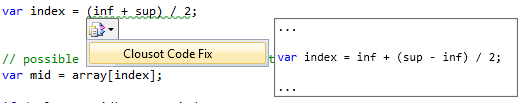
\includegraphics[width=\columnwidth]{./BinarySearchFix} 
\caption{The code repairs in the IDE.}
\label{fig:roslyn}
\end{figure}

\paragraph{IDE integration}
The goal of verified repairs is to use them interactively.
We integrated \Clousot\ in Visual Studio, via  the Microsoft Roslyn CTP~\cite{roslyn}.
An example of the user experience is  in~\refFig{roslyn}.
Roslyn exposes the C\# (and VB) compiler(s) as a service.
Plugins  register to Roslyn as code issues and code action providers.
\Clousot\ runs in background while the programmer is writing the program.
\Clousot\ reports the assertion violations as code issues.
For those assertions it can infer a code repair, \Clousot, reports it as a code action.
The code action is shown in a preview window.
The user choses to apply the code action or not.

Verified code repairs are realistic only if we can prove that the running time of the analysis + the generation of the fixes is small enough to be used in a real time programming environment.
On average \Clousot\ analyzes $6+$ methods per second and it infers $7.5$ repairs per second (\refFig{experience}).
The benchmarks above were run without any form of caching.
However, to further improve the performances, \Clousot\ has a built-in cache mechanism which let the analysis run only on the methods that have been modified since the last analysis.
In the past, we measured  the effects of the cache mechanism to at least a $10\times$ speed-up.

Overall, we are very positive that the approach can be applied during active development: code repairs + \Clousot\ with cache are efficient enough to be used in the IDE.


\section{Related Work}
\label{sec:related}


Automatic program repair is an active research subject in the testing
community~\cite{PezzeEtAl11}.  Starting from a program \code{P}
exposing a bug, the goal is to derive \code{P'} such that the bug is
repaired and no regression is introduced.  The repair is obtained by
pseudo-invariant inference~\cite{PerkinsEtAl09}, by genetic
algorithms~\cite{WeimerEtAl09,LeGouesEtAl-ICSE12}, by a smart exploration of the space of repairs~\cite{ChandraEtAl11}, or by instantiating some
templates~\cite{WeiEtAl}.  
Our approach is different in that we do not use a \emph{known} failing test to infer the repair (we start from a warning issued by the analyzer), we do not
need to run the program to apply our technique, the repair is inferred from the semantics of the program and it is verified.
In particular, the repairs we generate are property-specific, so our technique is not subject to the ``randomness'' in the proposed repairs of the aforementioned techniques.
Pex~\cite{Pex} uses symbolic execution to remove inputs that inevitably lead to an error.  
Our fixes are more general (\emph{e.g.}, we can fix overflowing expressions) and they soundly cope with loops -- symbolic execution engines do not infer loop invariants.
Starc~\cite{starc} mixes dynamic and static analysis to repair data structures.
We do tackle the problem of repairing data structures, but an interesting future research direction is to extend the definitions of Section~\ref{sec:verifiedrepairs} in that sense.
Samini~\emph{et al.}~\cite{SaminiEtAl-ICSE12} also combines dynamic and static analysis, but to repair PHP programs. 

Eclipse~\cite{eclipse} has a fix-it feature for repairing \emph{syntactically} wrong programs.
Whalen~\emph{et al.}~\cite{FITE} have a vision of an integrated \emph{test} environment.
Our vision is instead that of a \emph{semantic} integrated environment~\cite{LogozzoEtAlDemoOOPSLA12}, where a static analyzer runs in background, reports the errors, proposes the semantically justified repairs, and helps common programming tasks such as refactoring~\cite{CousotCousotLogozzoBarnett-OOPSLA12}, searching, code reviewing \emph{etc.}.

In the static analysis and verification community, recent work focused
on the repairing of Boolean
programs~\cite{SamantaEtAl08,JobstmannEtAl05,GriesmayerEtAl06}.  We
are not constrained to Boolean programs (we handle arbitrary C\#
programs), we handle infinite state spaces, and we have a very precise
yet universal notion of what a code repair is.  We were able to
generate repairs for the running examples of the above papers, with
the exception of the concurrent examples of~\cite{JobstmannEtAl05} -- \Clousot\ does not analyze parallel programs.  Surprisingly enough,
for the running example of~\cite{GriesmayerEtAl06} we inferred a
different repair (the initialization \code{x = 1}).


Other authors focused on repairing programs for  specific properties.
Martel~\cite{Martel09} tackles the problem of repairing \emph{floating} point arithmetic expressions.
The goal of~\cite{Martel09} is to infer (a good-enough approximation of) the most precise expression over machine floats equivalent to a given one.
His work is a code repair as according to our~\refDef{AssertionRepair}.
The main differences with the algorithm in~\refFig{OverflowFix} is that we focus on \code{ints}, so we are only interested in \emph{a} non-overflowing expression (there may be many in general), we perform online local rewriting instead of estimating the cost for the whole expression, we use all the numerical information inferred by the numerical abstract domains, not only the numerical ranges.

Vechev \emph{et al}~\cite{VechevEtAl10} present algorithms to introduce synchronization to remove bad interleavings.
In spirit, their approach is very similar to ours, as they use abstract interpretation to verify a program, and when they fail they gave themselves the freedom to modify the program also when it cannot be proven in the abstract that it is wrong (it may be correct in the concrete).
Apart from the handling of concurrency, the main difference is that we do not aim at applying the fixes automatically, we give some semantic guarantees on the repairs (they should not remove good runs and should increase the number of validated assertions), and we do not aim for minimality.

A related research field is the localization and the explanation of bugs and warnings.
Jose and Majumdar~\cite{JoseMajumdarPLDI11} present an algorithm to find the cause of a failing test.
Their approach is different from ours in many ways.
First, their algorithm requires the knowledge of a complete (failing) program execution -- we use static analysis instead.
Second, their error localization algorithm is based on finite techniques (bounded model checking, SAT, loops are handled by unrolling) so it is unlikely to cope with infinite state spaces as we do.
Third, their scope is to find the origin of the bug, whereas we aim at proposing a repair for a possible error in the program.
Rival~\cite{RivalSAS05} proposes a set of techniques to find the origin of alarms in an industrial strength static analyzer.
Our verified repairs can be also used to explain the origin of the warnings of the static analyzer.
Dillig, Dillig and Aiken~\cite{DilligDilligAiken-PLDI12} use abduction to infer the information a static analyzer is missing to carry on the correctness proof (or to prove the program is incorrect).
The information is presented to the user who should validate or refuse it.
We do not use abduction and we interact with the user by suggesting code changes, instead of logical formulas.
To see how our technique compares to abduction, we converted the C benchmarks of~\cite{DilligDilligAiken-PLDI12} into C\#.
We skipped those relying on C-specific patterns, \emph{e.g.}, string and pointer manipulation.
We applied~\clousot\ on the converted benchmarks.
For most of them, \clousot\ not even shows a suggestion, as it was able to prove the correctness without additional help.
For all the others, \emph{e.g.}, the one with real errors, \clousot\ suggested meaningfull assumptions and repairs.
Overall, we did not experience any advantage of the abduction technique of~\cite{DilligDilligAiken-PLDI12} over ours.


\section{Conclusions}
\label{sec:conclude}
We envision a future in which IDEs not only report semantic errors at design time but also suggest code repairs for them~\cite{LogozzoEtAlDemoOOPSLA12}.
This paper is a first step in that direction.
We introduced a new analysis for automatic, modular and verifiable
program repair.  We used abstract interpretation to formalize the
concepts of a verified repair (which removes bad runs while possibly
increasing good runs), and the weaker notion of verified
\emph{assertion} repair. We presented a set of verified repairs,
implemented in our static analyzer for .NET.  The repairs are
extracted from the semantic information computed by the abstract
interpreter.  

Experience shows that the repairs: (i) are generated
fast enough that they could be computed during active development; (ii)
cover almost  $4/5$ of the warnings raised; and (iii) are precise
enough to find new bugs for very well tested shipped libraries.



\section*{Acknowledgments}
We thank Andrew Bagel, Patrick and Radhia Cousot, Manuel F\"andrich, Matthieu Martel, Nikolai Tillman for the discussions.
We are also gratefull to Mike Barnett who made the Roslyn integration possible.

\bibliographystyle{plain}
\bibliography{bib}

\end{document}

